\documentclass{article}
\usepackage[spanish]{babel}
\usepackage{graphicx}
\usepackage{xcolor}
\usepackage[utf8]{inputenc}
\usepackage{fancyhdr}
\usepackage{lastpage}
\usepackage{enumitem}
\usepackage{listings}
\usepackage{float}

\pagestyle{fancy}
\fancyhf{}
\rfoot{Page \thepage\hspace{1pt} de~\pageref{LastPage}}

\title{Tarea Comunicación Indirecta}
\author{Guillermo López García}
\begin{document}
\maketitle

\textbf{1º Ejercicio.}\\
Uno de los motores CEP más famosos es el Proyecto Esper, creado por la empresa
EsperTech Inc. Esta implementado sobre Java Open Source y una de sus principales
ventajas respectos a otros motores CEP es que es código libre y además, al estar
implementado sobre Java, posee su capacidad multiplataforma. A continuación,
mostramos una imagen de su arquitectura de alto nivel y su modelo de procesamiento
y correlación.

\begin{figure}[H]
\centering
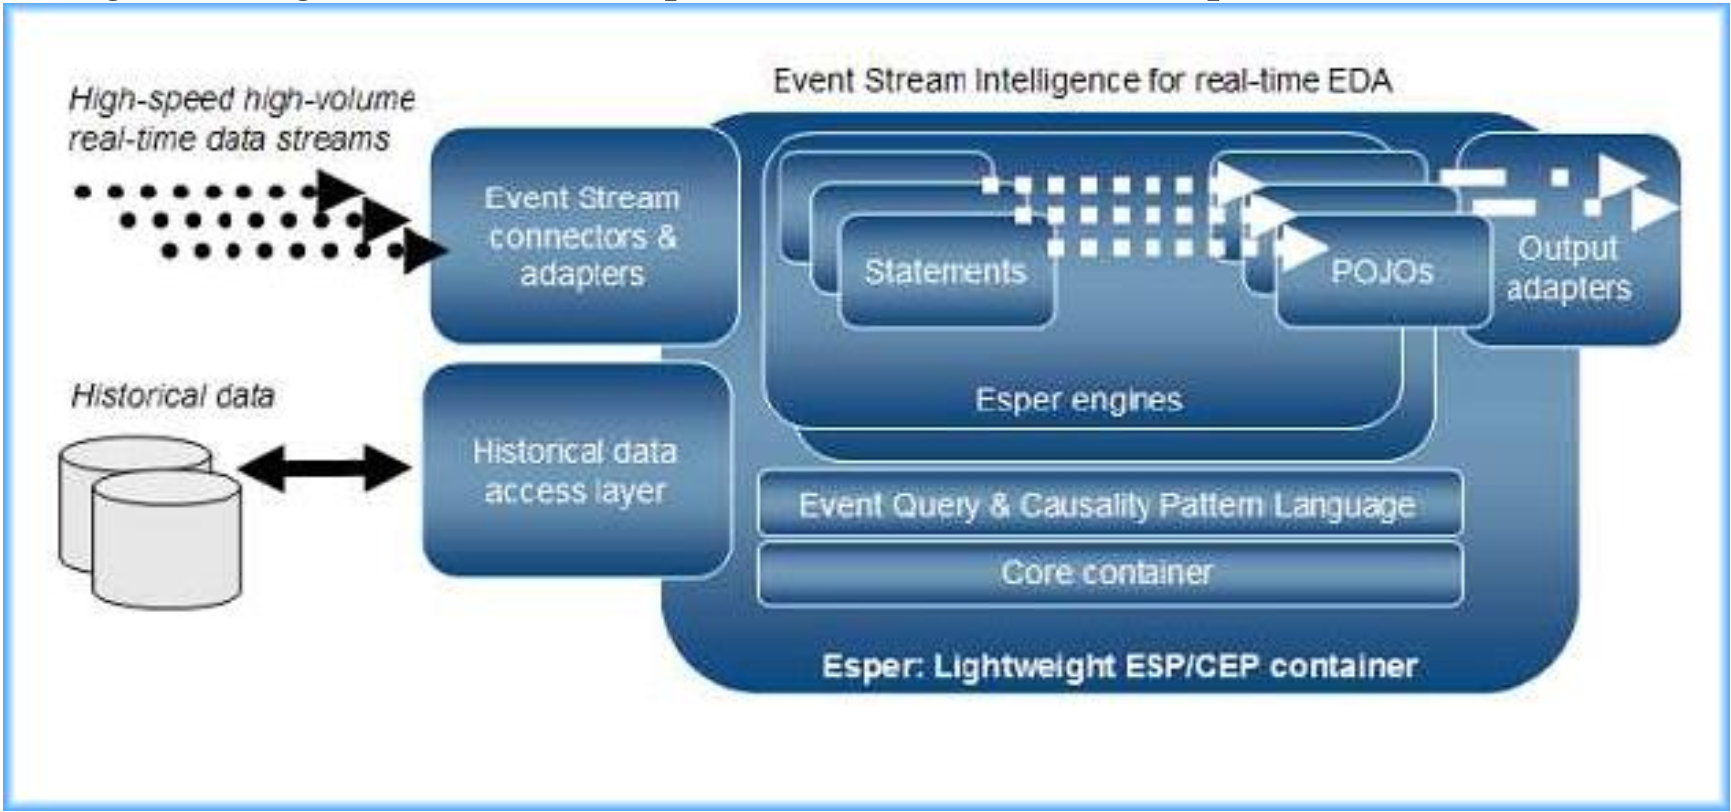
\includegraphics[width=0.7\linewidth]{./arquitectura_cep}
\caption{Arquitectura a alto nivel de Esper}
\end{figure}

\begin{figure}[H]
\centering
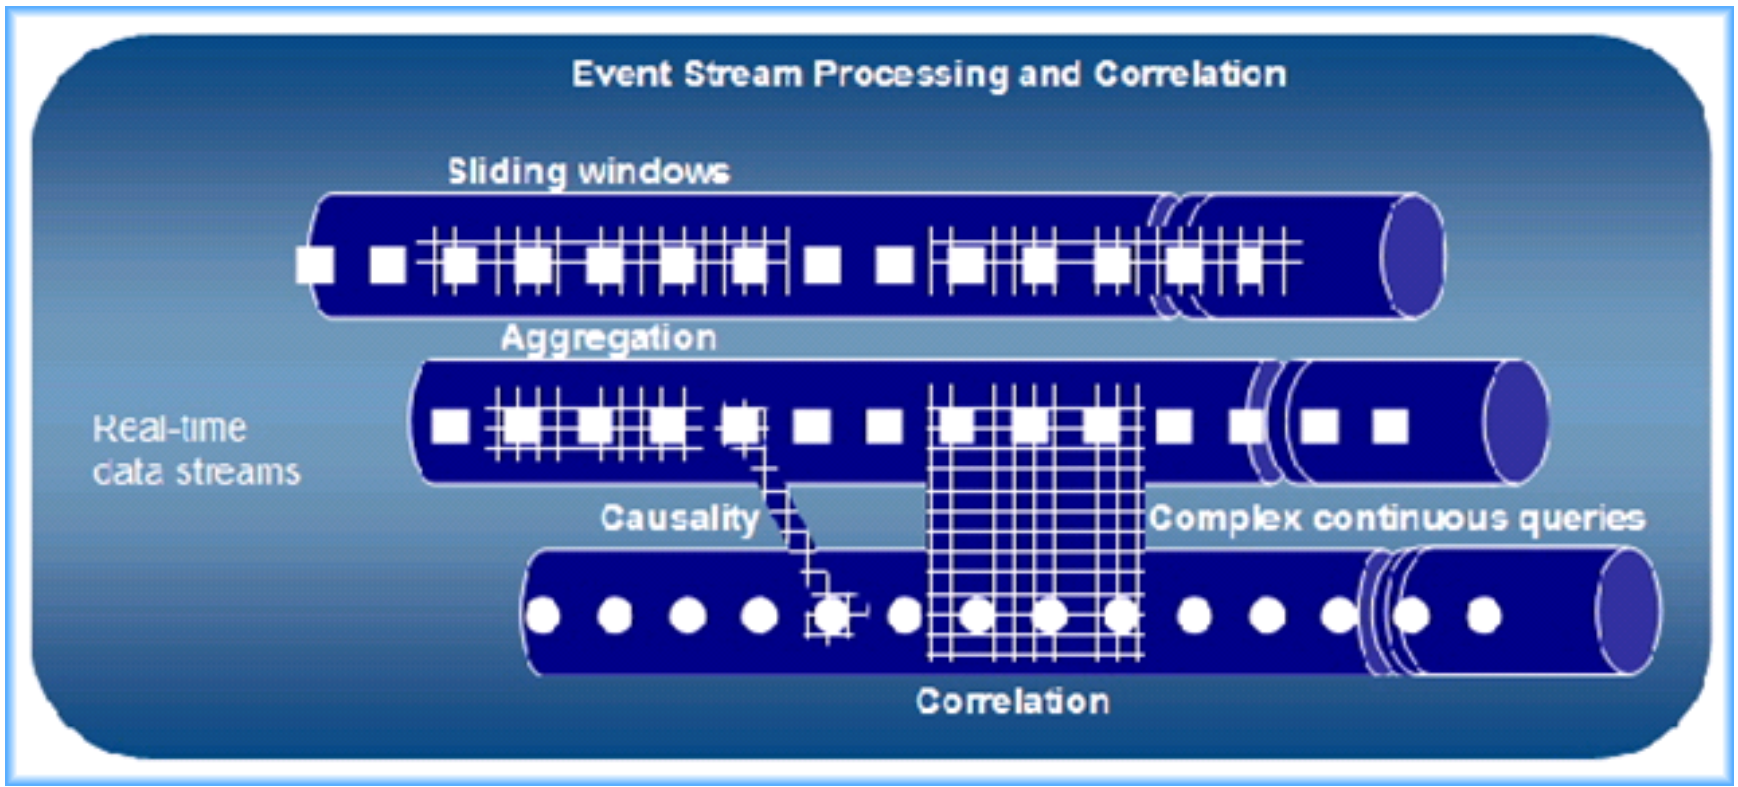
\includegraphics[width=0.7\linewidth]{./modelo_cep}
\caption{Modelo de Procesamiento y Correlación de Esper}
\end{figure}

\textbf{2º Ejercicio.}\\
JMS es una especificación de Java que define en esta plataforma una forma comunicación entre aplicaciones basada en el intercambio de mensajes. Los mensajes permiten a las aplicaciones no conocerse entre sí y comunicarse de forma asíncrona pudiendo hacer que los mensajes de una cola solo sean consumidos por un único receptor o por varios suscriptores interesados en un determinado tema. En el código de ejemplo muestro tanto la comunicación con colas (queues) como con temas (topics).
\\
A continuación, mostramos un ejemplo implementado en Java con un modelo Pub/Sub,
donde existen un publicador y dos suscriptores:

\lstset{
  language=Java,
  texcl=true,
  basicstyle=\ttfamily,
  columns=fullflexible,
  frame=single,
  breaklines=true,
  postbreak=\mbox{\textcolor{red}{$\hookrightarrow$}\space},
}
\begin{lstlisting}[frame=single]
// Clase Topic
package io.github.picodotdev.bitix.jms;

import java.util.Properties;

import javax.jms.Message;
import javax.jms.MessageListener;
import javax.jms.Session;
import javax.jms.TextMessage;
import javax.jms.TopicConnection;
import javax.jms.TopicConnectionFactory;
import javax.jms.TopicPublisher;
import javax.jms.TopicSession;
import javax.jms.TopicSubscriber;
import javax.naming.Context;
import javax.naming.InitialContext;

/**
 * Ejemplo que muestra como como enviar y recibir mensajes JMS de un Topic de forma remota.
 */
public class Topic {

    /**
     * Antes de ejecutar este ejemplo, usando WildFly se ha de crear un usuario guest y clave guest con el 
     * script WILDFLY_HOME/bin/add-user.sh.
     */
    public static void main(String[] args) throws Exception {
        // Usuario y password para conectarse al servidor JNDI y al Topic
     String usuario = "guest";
        String contrasena = "guest";

        // Propiedades para crear el contexto: clase factoría, url del servidor JNDI y credenciales
     Properties env = new Properties();
        env.put(Context.INITIAL_CONTEXT_FACTORY, "org.jboss.naming.remote.client.InitialContextFactory");
        env.put(Context.PROVIDER_URL, "http-remoting://localhost:8080");
        env.put(Context.SECURITY_PRINCIPAL, usuario);
        env.put(Context.SECURITY_CREDENTIALS, contrasena);

        // El objeto InitialContext permite obtener la referencias de los objetos registrado en el ábol JNDI
     InitialContext ic = new InitialContext(env);

        // Objetos a obtener para usar JMS: 
     // - TopicConnectionFactory
     // - TopicConection
     // - Topic
     // - TopicSession
     // - TopicSubscriber
     // - TopicPublisher
     TopicConnectionFactory connectionFactory = (TopicConnectionFactory) ic.lookup("jms/RemoteConnectionFactory");
        TopicConnection connection = connectionFactory.createTopicConnection(usuario, contrasena);
        
        // Obtener el Topic en el cual se publicarán y del cual se recibirán los mensajes
     javax.jms.Topic topic = (javax.jms.Topic) ic.lookup("jms/topic/test");

        // Preparar el publicador y subscriptor al Topic
     Subscriber subscriber1 = new Subscriber(connection, topic);
        Subscriber subscriber2 = new Subscriber(connection, topic);
        Publisher publisher = new Publisher(connection, topic);
        
        // Inicializar la recepción y envío de los mensajes
     connection.start();

        // Empezar a publicar mensajes en el Topic (y a recibirlos)
     Thread thread = new Thread(publisher);      
        thread.start();
        // Esperar a que el publicador termine de enviar mensajes
     thread.join();

        // Parar el envío y recepción de mensajes
     connection.stop();
        
        // Terminar liberando los recursos
     subscriber1.close();
        subscriber2.close();
        publisher.close();     
        connection.close();
        ic.close();
    }
    
    private static class Subscriber implements MessageListener {
        
        private TopicSession session;
        private TopicSubscriber subscriber;
        
        public Subscriber(TopicConnection connection, javax.jms.Topic topic) throws Exception {
            this.session = connection.createTopicSession(false, Session.AUTO_ACKNOWLEDGE);
            this.subscriber = this.session.createSubscriber(topic, null, false);
            this.subscriber.setMessageListener(this);
        }
        
        public void close() throws Exception  {
            subscriber.close();
            session.close();
        }
        
        @Override
        public void onMessage(Message message) {
            try {
                TextMessage text = (TextMessage) message;
                System.out.printf("Suscriptor (%s): El publicador dice: '%s'\n", this, text.getText());
            } catch (Exception e) {
                e.printStackTrace();
            }
        }
    }
    
    private static class Publisher implements Runnable {
        
        private TopicSession session;
        private TopicPublisher publisher;
        
        public Publisher(TopicConnection connection, javax.jms.Topic topic) throws Exception {
            this.session = connection.createTopicSession(false, Session.AUTO_ACKNOWLEDGE);
            this.publisher = this.session.createPublisher(topic);
        }
        
        public void close() throws Exception  {
            publisher.close();
            session.close();
        }
        
        @Override
        public void run() {
            try {
                for (int i = 0; i < 10; ++i) {
                    Message mensaje = session.createTextMessage(String.format("Hola mundo! (%d)", i));
                    publisher.publish(mensaje);
                    Thread.sleep(1000);
                }
            } catch (Exception e) {
                e.printStackTrace();
            }
        }
    }
}
\end{lstlisting}

\lstset{
  language=Java,
  texcl=true,
  basicstyle=\ttfamily,
  columns=fullflexible,
  frame=single,
  breaklines=true,
  postbreak=\mbox{\textcolor{red}{$\hookrightarrow$}\space},
}
\begin{lstlisting}[frame=single]
// Clase Queue
package io.github.picodotdev.bitix.jms;

import java.util.Properties;

import javax.jms.Message;
import javax.jms.MessageListener;
import javax.jms.QueueConnection;
import javax.jms.QueueConnectionFactory;
import javax.jms.QueueReceiver;
import javax.jms.QueueSender;
import javax.jms.QueueSession;
import javax.jms.Session;
import javax.jms.TextMessage;
import javax.naming.Context;
import javax.naming.InitialContext;

/**
 * Ejemplo que muestra como como enviar y recibir mensajes JMS de un Queue de forma remota.
 */
public class Queue {

    /**
     * Antes de ejecutar este ejemplo, usando WildFly se ha de crear un usuario guest y clave guest con el 
     * script WILDFLY_HOME/bin/add-user.sh.
     */
    public static void main(String[] args) throws Exception {
        // Usuario y password para conectarse al servidor JNDI y al Queue
     String usuario = "guest";
        String contrasena = "guest";

        // Propiedades para crear el contexto: clase factoría, url del servidor JNDI y credenciales
     Properties env = new Properties();
        env.put(Context.INITIAL_CONTEXT_FACTORY, "org.jboss.naming.remote.client.InitialContextFactory");
        env.put(Context.PROVIDER_URL, "http-remoting://localhost:8080");
        env.put(Context.SECURITY_PRINCIPAL, usuario);
        env.put(Context.SECURITY_CREDENTIALS, contrasena);

        // El objeto InitialContext permite obtener la referencias de los objetos registrado en el ábol JNDI
     InitialContext ic = new InitialContext(env);

        // Objetos a obtener para usar JMS: 
     // - QueueConnectionFactory
     // - QueueConection
     // - Queue
     // - QueueSession
     // - QueueSubscriber
     // - QueuePublisher
     QueueConnectionFactory connectionFactory = (QueueConnectionFactory) ic.lookup("jms/RemoteConnectionFactory");
        QueueConnection connection = connectionFactory.createQueueConnection(usuario, contrasena);
        
        // Obtener el Queue en el cual se publicarán y del cual se recibirán los mensajes
     javax.jms.Queue queue = (javax.jms.Queue) ic.lookup("jms/queue/test");

        // Preparar el publicador y subscriptor al Queue
     Receiver receiver1 = new Receiver(connection, queue);
        Receiver receiver2 = new Receiver(connection, queue);
        Sender sender = new Sender(connection, queue);
        
        // Inicializar la recepción y envío de los mensajes
     connection.start();

        // Empezar a enviar mensajes en el Queue (y a recibirlos)
     Thread thread = new Thread(sender);     
        thread.start();
        // Esperar a que el enviador termine de enviar mensajes
     thread.join();

        // Parar el envío y recepción de mensajes
     connection.stop();
        
        // Terminar liberando los recursos
     receiver1.close();
        receiver2.close();
        sender.close();        
        connection.close();
        ic.close();
    }
    
    private static class Receiver implements MessageListener {
        
        private QueueSession session;
        private QueueReceiver receiver;
        
        public Receiver(QueueConnection connection, javax.jms.Queue queue) throws Exception {
            this.session = connection.createQueueSession(false, Session.AUTO_ACKNOWLEDGE);
            this.receiver = this.session.createReceiver(queue);
            this.receiver.setMessageListener(this);
        }
        
        public void close() throws Exception  {
            receiver.close();
            session.close();
        }
        
        @Override
        public void onMessage(Message message) {
            try {
                TextMessage text = (TextMessage) message;
                System.out.printf("Receptor (%s): Un publicador dice: '%s'\n", this, text.getText());
            } catch (Exception e) {
                e.printStackTrace();
            }
        }
    }
    
    private static class Sender implements Runnable {
        
        private QueueSession session;
        private QueueSender sender;
        
        public Sender(QueueConnection connection, javax.jms.Queue queue) throws Exception {
            this.session = connection.createQueueSession(false, Session.AUTO_ACKNOWLEDGE);
            this.sender = this.session.createSender(queue);
        }
        
        public void close() throws Exception  {
            sender.close();
            session.close();
        }
        
        @Override
        public void run() {
            try {
                for (int i = 0; i < 10; ++i) {
                    Message mensaje = session.createTextMessage(String.format("Hola mundo! (%d)", i));
                    sender.send(mensaje);
                    Thread.sleep(1000);
                }
            } catch (Exception e) {
                e.printStackTrace();
            }
        }
    }
}
\end{lstlisting}

\end{document}
